\chapter{Solar flare detection}\label{solarFlareChapter}

Before developing the main solar flare detection algorithm a first study is presented targeting a powerful solar flare for which we knew the time of the event and therefore, the location of the Sun.

Although the aim of the main algorithm is detecting the solar flare without taking into consideration the position of the Sun, this study was done to understand how the core of the algorithm works: studying the correlation between the cosine of the solar-zenith angle and the detrended VTEC computed from the double-time difference of VTEC, hereinafter, the VTEC increase.

This chapter also provides an introduction to the formatting and use of the Global Navigation Satellite Systems data (GPS in this case) and how the main parameters necessary for the algorithms are computed.

\section{Data}

\subsection{GPS Data}

As we have seen in previous sections, the International GNSS Service (IGS) has made available open access GNSS data since its creation. The Crustal Dynamics Data Information System (CDDIS) is a central data archive for the NASA's Crustal Dynamics Project (CDP), dedicated to archiving space geodesy data for research. This archive has been storing and providing access to the GNSS data generated by the IGS since 1992.

Data is stored in the CDDIS server (\url{ftp://cddis.nasa.gov/gps/data/hourly/}). The files in this server contain raw GPS data that is then pre-processed to obtain the ambiguous STEC measurements, line-of-sight
geometry and detrended VTEC in the form of \textbf{ti} files. 



%\begin{figure}[!htb]
%	\begin{subfigure}[b]{0.3\textwidth}
%		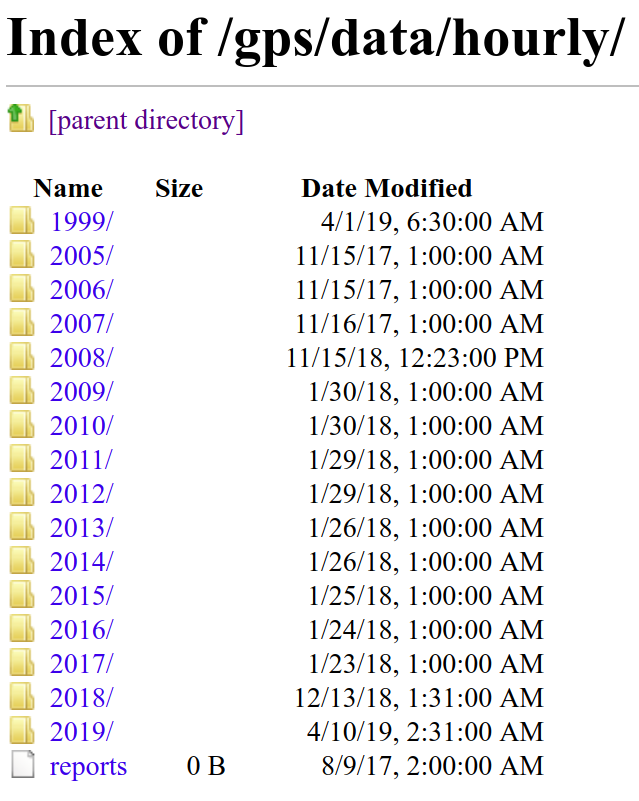
\includegraphics[width=\linewidth]{images/ch4/FTPNASA.png}
%		\caption{Files}
%	\end{subfigure}
%	\hfill
%	\begin{subfigure}[b]{0.5\textwidth}
%		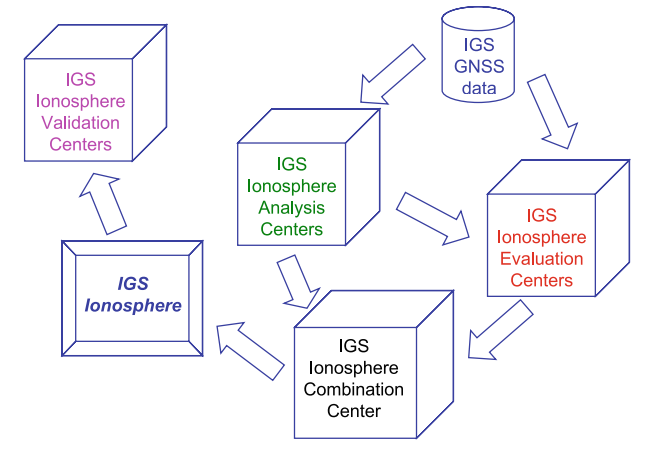
\includegraphics[width=\linewidth]{images/ch4/DataFlowIGS.png}
%		\caption{Data flow}
%	\end{subfigure}
%	\caption{CDDIS server (a) and data flow to obtain IGS data (b)}
%	\label{fig:exampleCDDIS}
%\end{figure}

However, for this and the following section, only the pre-processed ti files of past dates were needed, as detecting the flares in real time is a task that will be discussed later in the project, in which this pre-processing will have to be taken into consideration. The project supervisor, Manuel Hernández-Pajares, provided some of data sets to use as input for the algorithms, along with information about the formatting of this files.

\subsection{Formatting}

The ti files contain several rows of pre-processed GPS data. Each row has a Receiver Id. and a Transmitter Id., therefore, for each row we have the Ionospheric Pierce Point between the Receiver and Transmitter. Each IPP has several parameters that are relevant for our computations:

\begin{itemize}
\item The \textbf{GPS time}
\item The \textbf{Receiver Id.}
\item The \textbf{Transmitter Id.}
\item The \textbf{double time difference of Li}
\item The \textbf{ionospheric mapping function}, the approximate vertical-to-slant total electron content factor
\item The \textbf{right ascension} and \textbf{declination} of the IPP
\end{itemize}

\begin{minipage}{\linewidth}
\begin{lstlisting}[language=,caption=Format of the ti file]
Field number | Example value | Description
[...]
3 		0.008333333333		GPS time/hours (tsecdayobs/3600.d0)
4 		cand							Receiver Id.
5 		3									Transmitter Id.
[...]
21 		-0.5131586E-02		d2li
[...]
43 		0.1565765332E+01		xmapping_ion
44 		334.449							xraion
45 		33.092							xlation
[...]
\end{lstlisting}
\end{minipage}
The files also contain the right ascension and declination of the \textbf{Sun}, which will be used in the last chapters to study the error of the algorithm's estimations of the source's position.

\subsection{The Halloween Solar Storm: X17.2 flare}

First, the data set we used was that of the so-called Halloween Storm, a powerful geomagnetic storm that took place from October to early November in the year 2003. In particular, we will try to replicate the results shown in figure \ref{fig:halloweenPaper}, shown in the paper \textit{"GNSS measurement of EUV photons flux rate during strong and mid solar flares"} for a poweful flare that took place in October 28th, 2003 \cite{hernandez2012gnss}.

\begin{figure}[!htb]
	\begin{centering}
		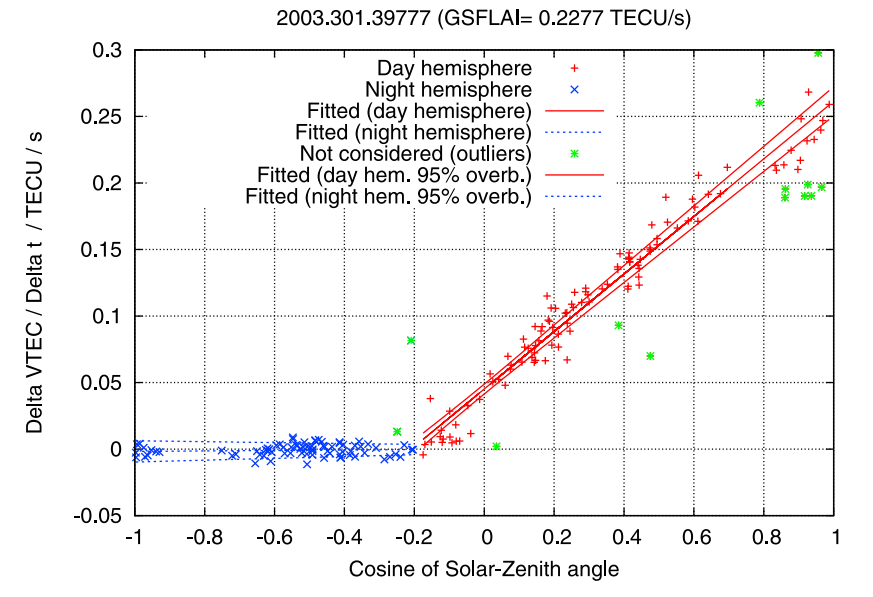
\includegraphics[width=0.5\linewidth]{images/ch4/halloweenPaper.png}
		\caption{VTEC as a function of the cosine of the solar-zenith angle}
		\label{fig:halloweenPaper}
	\end{centering}
\end{figure}

As we can see the plot of the flare called X17.2 took place exactly at 2003.301.39777 (year.day.seconds of GPS time). In hours, 39777 seconds of a day is $39777s * 1h/3600s = 11.049...h$, around 11AM. 

The ti files provided contained data from 10.5h to 11.5h (with a sampling rate of 30 seconds), so that we could see the VTEC distribution throughout the day.

With this data we can compute the two parameters that will yield the plot shown in figure \ref{fig:halloweenPaper}: the detrended \textbf{VTEC value} and the \textbf{cosine of the solar-zenith angle}, i.e. solar-IPP angle.

\section{Vertical Total Electron Content (VTEC)}

Fisrt we wanted to obtain the VTEC distribution throughout the day, to visually see if any spikes appeared confirming that the moment we were going to study based on the paper was correct.

For each epoch in our data set (from 10.5 to 11.5 with a sampling rate of 30 seconds) we needed to compute an estimation of the VTEC value.

\subsection{Computing the VTEC}

As we have mentioned before, one of the main paramenters relevant to the computation is the \textbf{double time difference of LI}, the d2li field in the ti file. The Li is the "ionospheric combination of carrier phases" \cite{hernandez2012gnss}, a direct measurement of TEC. Because this is proportional to the double derivative, with the following operation we obtain \textbf{curvature of the VTEC}, which is proportional to the detrenteded VTEC, this will be observed in figure \ref{fig:vtecDistribution}.

This value can be estimated using the following operation:

\begin{equation} \label{eq:1}
	d^{2}V = \frac{d^{2}Li}{M} = -2 * \frac{(LI(t) - \frac{(LI(t-dt)+ LI(t+dt))}{2})}{M}
\end{equation}

Where $M=\frac{1}{\cos Z}$ is the "ionospheric mapping function", the inverse of the cosine of the satellite-zenith angle that we have for each IPP. \cite{hernandez2012gnss}. This is the \textbf{xmappingion} field in the ti file.

Although the data that will be used throughout the project is going to be the curvature of the detrended VTEC, it will be referenced simply as VTEC from now on for readability. This value indicates whether a point is a maximum or a minimum, so it can work as an indicator of the VTEC.

\paragraph{Implementation}

Below is the code used to compute the VTEC value in Fortran that we will use to replicate the plot from figure \ref{fig:halloweenPaper}.

\begin{minipage}{\linewidth}
\begin{lstlisting}[language=Fortran, caption=Simple Fortran function to compute the VTEC value]
double precision function estimateVTEC (mapIon, d2Li)
	implicit none
	double precision, intent(in) :: mapIon, d2Li
	double precision :: vtec
	
	vtec = d2Li/mapIon
	return
end function estimateVTEC
\end{lstlisting}
\end{minipage}

\subsection{Distribution throughout the day}

Because the only operation that had to be performed was the previous division, a simple AWK script was used to filter the two necessary fields from the data file and print the resulting value as well as its time. 

\begin{minipage}{\linewidth}
\begin{lstlisting}[language=Awk, caption=AWK script to estimate the VTEC]
{
	/a/
	d2li = $21;
	mappingFunc = $43;
	vtec = d2li/mappingFunc;
	print $3 " " vtec
}
\end{lstlisting}
\end{minipage}

\begin{minipage}{\linewidth}
\begin{lstlisting}[language=Bash, caption=Bash script to execute the procedures]
#!/bin/bash
tiDataFile="../data/ti.2003.301.10h30m-11h30m.gz"

zcat "$tiDataFile" | gawk -f previewVTECDistribution.awk > vtecValues
gnuplot -e "set terminal png; set output 'vtecDistribution.png'; set title 'VTEC Distribution'; set xlabel 'Time of the day (hours)'; set ylabel 'VTEC'; set grid; plot \"vtecValues\" using 1:2 with point"
\end{lstlisting}
\end{minipage}


The bash script executes the AWK process with the data as the input and outputs \textit{n} rows with two columns: the \textbf{time of the day} and the \textbf{calculated VTEC}, and finally plots the results using Gnuplot. 

\begin{figure}[!htb]
	\begin{centering}
		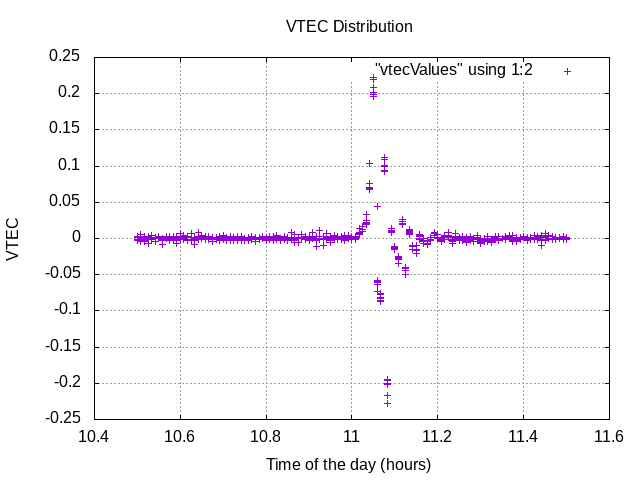
\includegraphics[width=0.5\linewidth]{images/ch4/vtecDistributionVill.png}
		\caption{VTEC distribution throughout the day for IPPs that have Vill as the receiver}
		\label{fig:vtecDistribution}
	\end{centering}
\end{figure}

Visually, a spike can be seen between 11 and 11.2 hours. To see the event more clearly, though, we can focus on one specific receiver (which will still yield multiple IPPs, as the receiver works with different satellites). For the particular case of the Villafranca, Spain station (identified as Vill in the ti files), we obtain the plot from figure \ref{fig:vtecDistribution}. At this time of the day around 11:00h the Sun would have a greater effect on the IPPs of this station due to its location close to the zenith, so the spike can be seen more clearly. 

As mentioned before, the flare took place at 11.05, so we could proceed using the studied data range and this epoch in particular.



%\begin{figure}[!htb]
%	\begin{subfigure}[b]{0.5\textwidth}
%		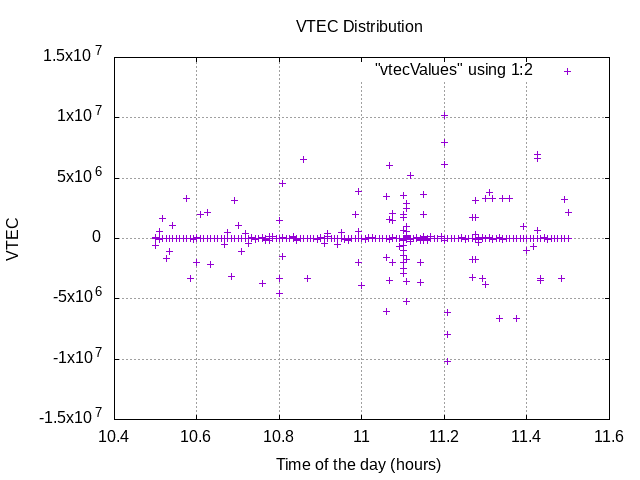
\includegraphics[width=\linewidth]{images/ch4/vtecDistributionGeneral.png}
%		\caption{All IPPs}
%	\end{subfigure}
%	\hfill
%	\begin{subfigure}[b]{0.5\textwidth}
%		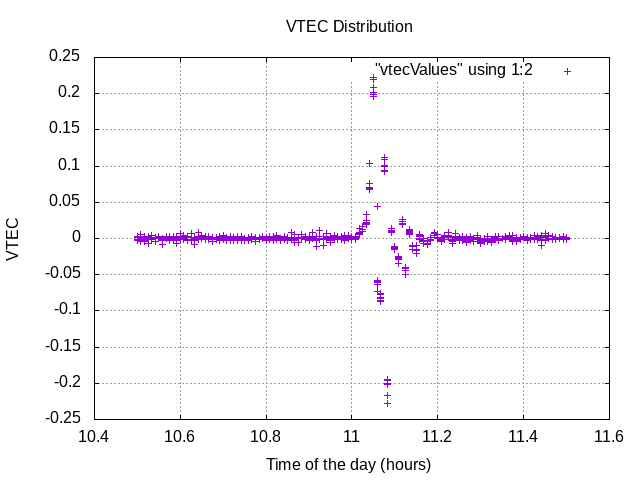
\includegraphics[width=\linewidth]{images/ch4/vtecDistributionVill.png}
%		\caption{Villafranca station}
%	\end{subfigure}
%	\caption{VTEC distribution throughout the day for all IPPS (a) and for IPPs that have Vill as the receiver (b)}
%	\label{fig:vtecDistribution}
%\end{figure}

\section{Solar-zenith angle}

The solar-zenith angle (denoted $\chi$ from now onward) plays a major role when studying this event: it is the angle formed by the Sun and the Earth's zenith and indicates the effect the flare is having on a particular IPP. It is expected that this variable presents a correlation with the increase in VTEC with an scaling factor proportional to the source EUV flux rate drift \cite{hernandez2012gnss}, which is what we aim to observe in this chapter.

Figure \ref{fig:solar-zenith-angle}, at the end of the chapter, provides a visual representation of this variable that along with the results depicts how it can affect the VTEC value. 

Right Ascension and Declination are two concepts similar to longitude and latitude, respectively, used to describe the location of objects in the sky, in particular in a sphere of infinite radius with the Earth as its center called the \textbf{celestial sphere}.

Taking this into account, Right Ascension play the role of longitude, but referred to the Aries point, expressed in degrees (or more commonly in hours, minutes and seconds) and Declination, the equivalent of latitude, is expressed in degrees between the two poles: +90$^{\circ}$ and -90$^{\circ}$, this reference system is used to describe the position of objects in the sky. \cite{nasareferencesystem}

The angle $\beta$ between two celestial objects is obtained by means of equations \ref{eq:3}, \ref{eq:4} and \ref{eq:5}, by performing the dot product of the two unit vectors that define the position of the objects using their right ascension ($\alpha$) and declination ($\delta$).

\begin{equation} \label{eq:3}
unitVectorObjectA =	
\begin{bmatrix}
\cos\delta_{g} * \cos\alpha_{g} \\ 
\cos\delta_{g} * \sin\alpha_{g} \\
\sin\delta_{g}
\end{bmatrix}
\end{equation}

\begin{equation} \label{eq:4}
unitVectorObjectB =	
\begin{bmatrix}
\cos\delta_{s} * \cos\alpha_{s} \\ 
\cos\delta_{s} * \sin\alpha_{s} \\
\sin\delta_{s}
\end{bmatrix}
\end{equation}

\begin{equation} \label{eq:5}
\cos \beta = unitVectorObjectA \cdot unitVectorObjectB
\end{equation}\\

For this case, the cosine of the solar-zenith angle $\chi$ is computed using the IPP's Right Ascension and Latitude (equivalent to declination). The previous dot product can be simplified to:

\begin{equation} \label{eq:6}
\cos \chi = \sin\delta_{IPP}*\sin\delta_{Sun} + \cos\delta_{IPP}*\cos\delta_{Sun}*\cos(\alpha_{IPP} - \alpha_{Sun})
\end{equation}\\

The following FORTRAN code is the function that implements equation \ref{eq:6} and returns $\cos \chi$ (given both angles in radians):

\begin{minipage}{\linewidth}
\begin{lstlisting}[language=Fortran, caption=Computation of the solar-zenith a angle's cosine]
double precision function computeAngle (raIPP, decIPP, raSun, decSun)
	implicit none
	double precision, intent(in) :: raIPP, decIPP, raSun, decSun
	double precision :: solarZenithAngle
	
	solarZenithAngle = sin(decIPP)*sin(decSun) + cos(decIPP)*cos(decSun)*cos(raIPP - raSun)
	return
end function computeAngle
\end{lstlisting}
\end{minipage}

\section{Results}

Taking $212.338^{\circ}$ and $-13.060^{\circ}$ as the corresponding Sun's right ascension and declination, respectively, and the measurements of all IPPs at 11.05 hours, figure \ref{fig:results} shows the plot of the output of our program.

\begin{figure}[!htb]
\begin{centering}
	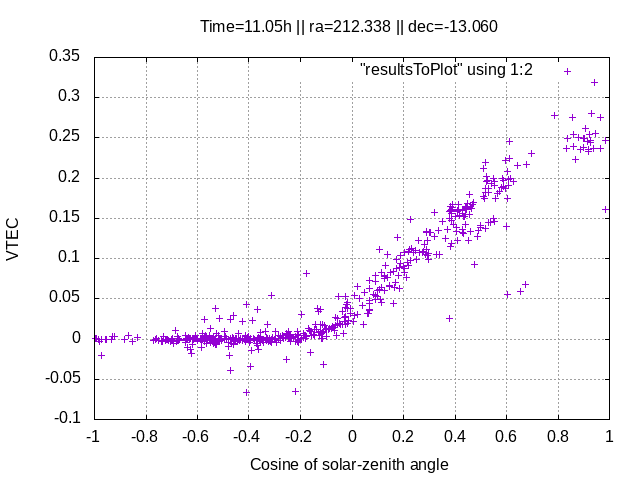
\includegraphics[width=0.5\linewidth]{images/ch4/resultSunTest.png}
	\caption{VTEC value as a function of the solar-zenith angle cosine}
	\label{fig:results}
\end{centering}
\end{figure}

As we can observe, the resulting plot, similar to the one from figure \ref{fig:halloweenPaper}, shows a strong corelation between the cosine of the solar-zenith angle and the VTEC content, which increases from $\cos\chi = -0.1$ to $\cos\chi = 1$ (90$^{\circ}$) (the effect of the Sun on the IPP increases) and it does not seem to be affected from $\cos\chi = -1$ (180$^{\circ}$) to $\cos\chi = -0.1$ (when the IPP is in the night hemisphere).

In conclusion, we can see that there appears to be the expected correlation between the two variables. This correlation will be studied in more detail in the following section, where a first approach of the algorithm will be presented to detect the flare without knowing the location of its source.













